%%%%%%%%%%%%%%%%%%%%%%%%%%%%%%%%%%%%%%%%%%%%%%%%%%%%%%%%%%%%%%%%%%%%%
%% This is a (brief) model paper using the achemso class
%% The document class accepts keyval options, which should include
%% the target journal and optionally the manuscript type.
%%%%%%%%%%%%%%%%%%%%%%%%%%%%%%%%%%%%%%%%%%%%%%%%%%%%%%%%%%%%%%%%%%%%%
\documentclass[journal=jacsat,manuscript=article]{achemso}

%%%%%%%%%%%%%%%%%%%%%%%%%%%%%%%%%%%%%%%%%%%%%%%%%%%%%%%%%%%%%%%%%%%%%
%% Place any additional packages needed here.  Only include packages
%% which are essential, to avoid problems later. Do NOT use any
%% packages which require e-TeX (for example etoolbox): the e-TeX
%% extensions are not currently available on the ACS conversion
%% servers.
%%%%%%%%%%%%%%%%%%%%%%%%%%%%%%%%%%%%%%%%%%%%%%%%%%%%%%%%%%%%%%%%%%%%%
\usepackage[version=3]{mhchem} % Formula subscripts using \ce{}

%%%%%%%%%%%%%%%%%%%%%%%%%%%%%%%%%%%%%%%%%%%%%%%%%%%%%%%%%%%%%%%%%%%%%
%% If issues arise when submitting your manuscript, you may want to
%% un-comment the next line.  This provides information on the
%% version of every file you have used.
%%%%%%%%%%%%%%%%%%%%%%%%%%%%%%%%%%%%%%%%%%%%%%%%%%%%%%%%%%%%%%%%%%%%%
%%\listfiles

%%%%%%%%%%%%%%%%%%%%%%%%%%%%%%%%%%%%%%%%%%%%%%%%%%%%%%%%%%%%%%%%%%%%%
%% Place any additional macros here.  Please use \newcommand* where
%% possible, and avoid layout-changing macros (which are not used
%% when typesetting).
%%%%%%%%%%%%%%%%%%%%%%%%%%%%%%%%%%%%%%%%%%%%%%%%%%%%%%%%%%%%%%%%%%%%%
\newcommand*\mycommand[1]{\texttt{\emph{#1}}}

%%%%%%%%%%%%%%%%%%%%%%%%%%%%%%%%%%%%%%%%%%%%%%%%%%%%%%%%%%%%%%%%%%%%%
%% Meta-data block
%% ---------------
%% Each author should be given as a separate \author command.
%%
%% Corresponding authors should have an e-mail given after the author
%% name as an \email command. Phone and fax numbers can be given
%% using \phone and \fax, respectively; this information is optional.
%%
%% The affiliation of authors is given after the authors; each
%% \affiliation command applies to all preceding authors not already
%% assigned an affiliation.
%%
%% The affiliation takes an option argument for the short name.  This
%% will typically be something like "University of Somewhere".
%%
%% The \altaffiliation macro should be used for new address, etc.
%% On the other hand, \alsoaffiliation is used on a per author basis
%% when authors are associated with multiple institutions.
%%%%%%%%%%%%%%%%%%%%%%%%%%%%%%%%%%%%%%%%%%%%%%%%%%%%%%%%%%%%%%%%%%%%%
\author{Elliott Capek}
\altaffiliation{Department of Biochemistry, Oregon State University}
%% \author{}
%% \altaffiliation{}
%% \author{}
%% \altaffiliation{}
%% \email{}
%% \phone{}
%% \fax{}
%% \affiliation[]{}
%% \alsoaffiliation[]{}
%% \author{}
%% \email{}
%% \affiliation[]{}
\author{Aidan Estelle}
\affiliation[]{}
\alsoaffiliation[]{}

%%%%%%%%%%%%%%%%%%%%%%%%%%%%%%%%%%%%%%%%%%%%%%%%%%%%%%%%%%%%%%%%%%%%%
%% The document title should be given as usual. Some journals require
%% a running title from the author: this should be supplied as an
%% optional argument to \title.
%%%%%%%%%%%%%%%%%%%%%%%%%%%%%%%%%%%%%%%%%%%%%%%%%%%%%%%%%%%%%%%%%%%%%
\title[]{Click chemistry reveals an alternate mechanism for HPII catalase}

%%%%%%%%%%%%%%%%%%%%%%%%%%%%%%%%%%%%%%%%%%%%%%%%%%%%%%%%%%%%%%%%%%%%%
%% Some journals require a list of abbreviations or keywords to be
%% supplied. These should be set up here, and will be printed after
%% the title and author information, if needed.
%%%%%%%%%%%%%%%%%%%%%%%%%%%%%%%%%%%%%%%%%%%%%%%%%%%%%%%%%%%%%%%%%%%%%
\abbreviations{IR,NMR,UV}
\keywords{American Chemical Society, \LaTeX}

\begin{document}
%%%%%%%%%%%%%%%%%%%%%%%%%%%%%%%%%%%%%%%%%%%%%%%%%%%%%%%%%%%%%%%%%%%%%
%% The manuscript does not need to include \maketitle, which is
%% executed automatically.  The document should begin with an
%% abstract, if appropriate.  If one is given and should not be, the
%% contents will be gobbled.
%%%%%%%%%%%%%%%%%%%%%%%%%%%%%%%%%%%%%%%%%%%%%%%%%%%%%%%%%%%%%%%%%%%%%
\begin{abstract}
  %% This is an example document for the \textsf{achemso} document
  %% class, intended for submissions to the American Chemical Society
  %% for publication. The class is based on the standard \LaTeXe\
  %% \textsf{report} file, and does not seek to reproduce the appearance
  %% of a published paper.

  %% This is an abstract for the \textsf{achemso} document class
  %% demonstration document.  An abstract is only allowed for certain
  %% manuscript types.  The selection of \texttt{journal} and
  %% \texttt{manuscript} will determine if an abstract is valid.  If
  %% not, the class will issue an appropriate error.
\end{abstract}

%%%%%%%%%%%%%%%%%%%%%%%%%%%%%%%%%%%%%%%%%%%%%%%%%%%%%%%%%%%%%%%%%%%%%
%% Start the main part of the manuscript here.
%%%%%%%%%%%%%%%%%%%%%%%%%%%%%%%%%%%%%%%%%%%%%%%%%%%%%%%%%%%%%%%%%%%%%
\section{Introduction}

\section{Methods}
\textbf{Protein expression}\\
Wildtype protein was expressed by transforming the pBAD-HPII-WT plasmid in Figure \ref{fig:pbad-hpii-wt} into competent \textit{E. coli} DH10B cells via heat-shock. Plasmid includes ampicillin resistance and a 6xHis tag on the N-term of the HPII gene. Cells were then grown in autoinduction media with an arabinose inducer (0.1\% aspartate pH 7.5, 0.2\% glycerol, mineral salts, 0.05\% glucose, 20mM MgSO4, 0.05\% arabinose, trace metals and AA mix) for 48 hours, shaking, at 37C. Cells were then pelletized and stored at -80C.\\

\textbf{Protein purification}\\
Pelletized cells were reconstituted in TALON equilibration buffer (50mM sodium phosphate, 300mM NaCl) and microfluidized, also in equilibration buffer. Lysed cells were spun down at 15K RPM for 20 minutes at 4C. Supernatant was collected and combined with 300$\mu L$ bed volume TALON beads per 100mL cultured cells. TALON-supernatant mix was nutated for 30 minutes at 4C. Bound beads were then spun down at 500g for 5 minutes and the supernatant discarded. The beads were applied to a pre-washed gravity-flow column at RT and washed twice with 10mL equilibration buffer. Elution was done using 2mL elution buffer (50mM sodium phosphate, 300mM NaCl, 250mM imidazole) into four 500$\mu L$ aliquots. Protein was then stored at 4C.\\

\section{Results and discussion}

\begin{figure}
\centering
\includegraphics[width=\linewidth]{figures/crude-wt-gel}
\caption{Electrophoresis gel of wildtype expression. Serial dillution of WT protein purification shown in two lanes. Major band in purification lanes correspond to protein of approximately 75kD, as expected for catalse single subunit.}
\label{fig:duration-length}
\end{figure}

\subsection{Outline}

\subsection{References}

\cite{Mena2000,Abernethy2003,Friedman-Hill2003,EuropeanCommission2008}.

\bibnote{This is a note. The text will be moved the the references section.  The title of the section will change to ``Notes and References''.}

\textsf{natbib}

\citeauthor{Abernethy2003}
\textsf{natbib}
\citeyear{Cotton1999}
~\citenum{Mena2000}
\cite{Pople2003}
\textsf{natbib}
\texttt{achemso-demo.bib}
\latin{et al.}
\texttt{\textbackslash latin}
\textsf{mciteplus}
\cite{Johnson1972,*Arduengo1992,*Eisenstein2005,*Arduengo1994}
\texttt{\textbackslash mciteSubRef}
\mciteSubRef{Eisenstein2005}
\cite[p.~1]{Cotton1999}.

%%%%%%%%%%%%%%%%%%%%%%%%%%%%%%%%%%%%%%%%%%%%%%%%%%%%%%%%%%%%%%%%%%%%%
%% The same is true for Supporting Information, which should use the
%% suppinfo environment.
%%%%%%%%%%%%%%%%%%%%%%%%%%%%%%%%%%%%%%%%%%%%%%%%%%%%%%%%%%%%%%%%%%%%%
\begin{suppinfo}

\end{suppinfo}

%%%%%%%%%%%%%%%%%%%%%%%%%%%%%%%%%%%%%%%%%%%%%%%%%%%%%%%%%%%%%%%%%%%%%
%% The appropriate \bibliography command should be placed here.
%% Notice that the class file automatically sets \bibliographystyle
%% and also names the section correctly.
%%%%%%%%%%%%%%%%%%%%%%%%%%%%%%%%%%%%%%%%%%%%%%%%%%%%%%%%%%%%%%%%%%%%%
\bibliography{references}

%%%%%%%%%%%%%%%%%%%%%%%%%%%%%%%%%%%%%%%%%%%%%%%%%%%%%%%%%%%%%%%%%%%%%
%% The "tocentry" environment can be used to create an entry for the
%% graphical table of contents.
%%%%%%%%%%%%%%%%%%%%%%%%%%%%%%%%%%%%%%%%%%%%%%%%%%%%%%%%%%%%%%%%%%%%%

%% \begin{tocentry}

%% \end{tocentry}

\end{document}


results section mantra:
1 - Explain what you did and then describe what you expected as an outcome
2 - Describe the data and show the dta
3 - Interpret the data
